\let\negmedspace\undefined
\let\negthickspace\undefined
\documentclass[journal]{IEEEtran}
\usepackage[a5paper, margin=10mm, onecolumn]{geometry}
%\usepackage{lmodern} % Ensure lmodern is loaded for pdflatex
\usepackage{tfrupee} % Include tfrupee package
\setlength{\headheight}{1cm} % Set the height of the header box
\setlength{\headsep}{0mm}     % Set the distance between the header box and the top of the text
\usepackage{gvv-book}
\usepackage{gvv}
\usepackage{cite}
\usepackage{amsmath,amssymb,amsfonts,amsthm}
\usepackage{algorithmic}
\usepackage{graphicx}
\usepackage{textcomp}
\usepackage{xcolor}
\usepackage{txfonts}
\usepackage{listings}
\usepackage{enumitem}
\usepackage{mathtools}
\usepackage{gensymb}
\usepackage{comment}
\usepackage[breaklinks=true]{hyperref}
\usepackage{tkz-euclide} 
\usepackage{listings}
% \usepackage{gvv}                                        
\def\inputGnumericTable{}                                 
\usepackage[latin1]{inputenc}                                
\usepackage{color}                                            
\usepackage{array}                                            
\usepackage{longtable}                                       
\usepackage{calc}                                             
\usepackage{multirow}                                         
\usepackage{hhline}                                           
\usepackage{ifthen}                                           
\usepackage{lscape}
\usepackage{circuitikz}
\tikzstyle{block} = [rectangle, draw, fill=blue!20, 
    text width=4em, text centered, rounded corners, minimum height=3em]
\tikzstyle{sum} = [draw, fill=blue!10, circle, minimum size=1cm, node distance=1.5cm]
\tikzstyle{input} = [coordinate]
\tikzstyle{output} = [coordinate]
\begin{document}

\begin{center}
\textbf{\Large Digital Thermometer}
\end{center}

\hfill Balu - A125BTECH11017 \\
\hfill Manohar - A125BTECH11028 \\[1cm]

\textbf{AIM :}

The objective of this project is to design and implement a digital thermometer that
measures temperature using a PT-100 Resistance Temperature Detector (RTD), Processes
the signal through an Arduino microcontroller, and Displays the Temperature on a 16x2
LCD. The Temperature is Determined using linear regression (least squares method).

\vspace{1cm}

\textbf{Components:}
\begin{itemize}
    \item PT-100 RTD
    \item Arduino Uno
    \item Jumper wires
    \item Bread board
    \item Potentiometer
    \item LCD (16x2)
    \item 100$\Omega$ Resistor
\end{itemize}
\section*{Procedure:}

\begin{enumerate}
    \item Build the circuit.
    \item Write arduino code to measure voltage.
    \item Take data set of temperature and voltage using thermometer.
    \item Callendos Van dusen equations.
    \begin{enumerate}
        \item $V = n_0 + n_1T + n_2T^2$
        \item $T = a_0 + a_1V + a_2V^2$
    \end{enumerate}
    \item Use least squaees method on data set and find the coefficients.
    \item Vulidate this model using 10 data points (T, V).
    \item Calculate Mean Absolute essor (M.A.E) and analyze parameters.
\end{enumerate}
\begin{figure}[h]
    \centering
    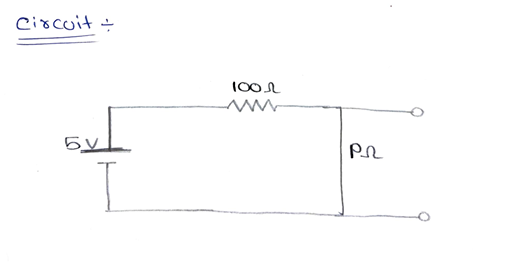
\includegraphics[width=0.5\linewidth]{figs/Screenshot 2025-11-01 at 00-44-18 Adobe Scan 31 Oct 2025 (1) - Adobe cloud storage.png}
    \caption{Circuit}
    \label{fig:placeholde}
\end{figure}
\begin{figure}[h]
    \centering
    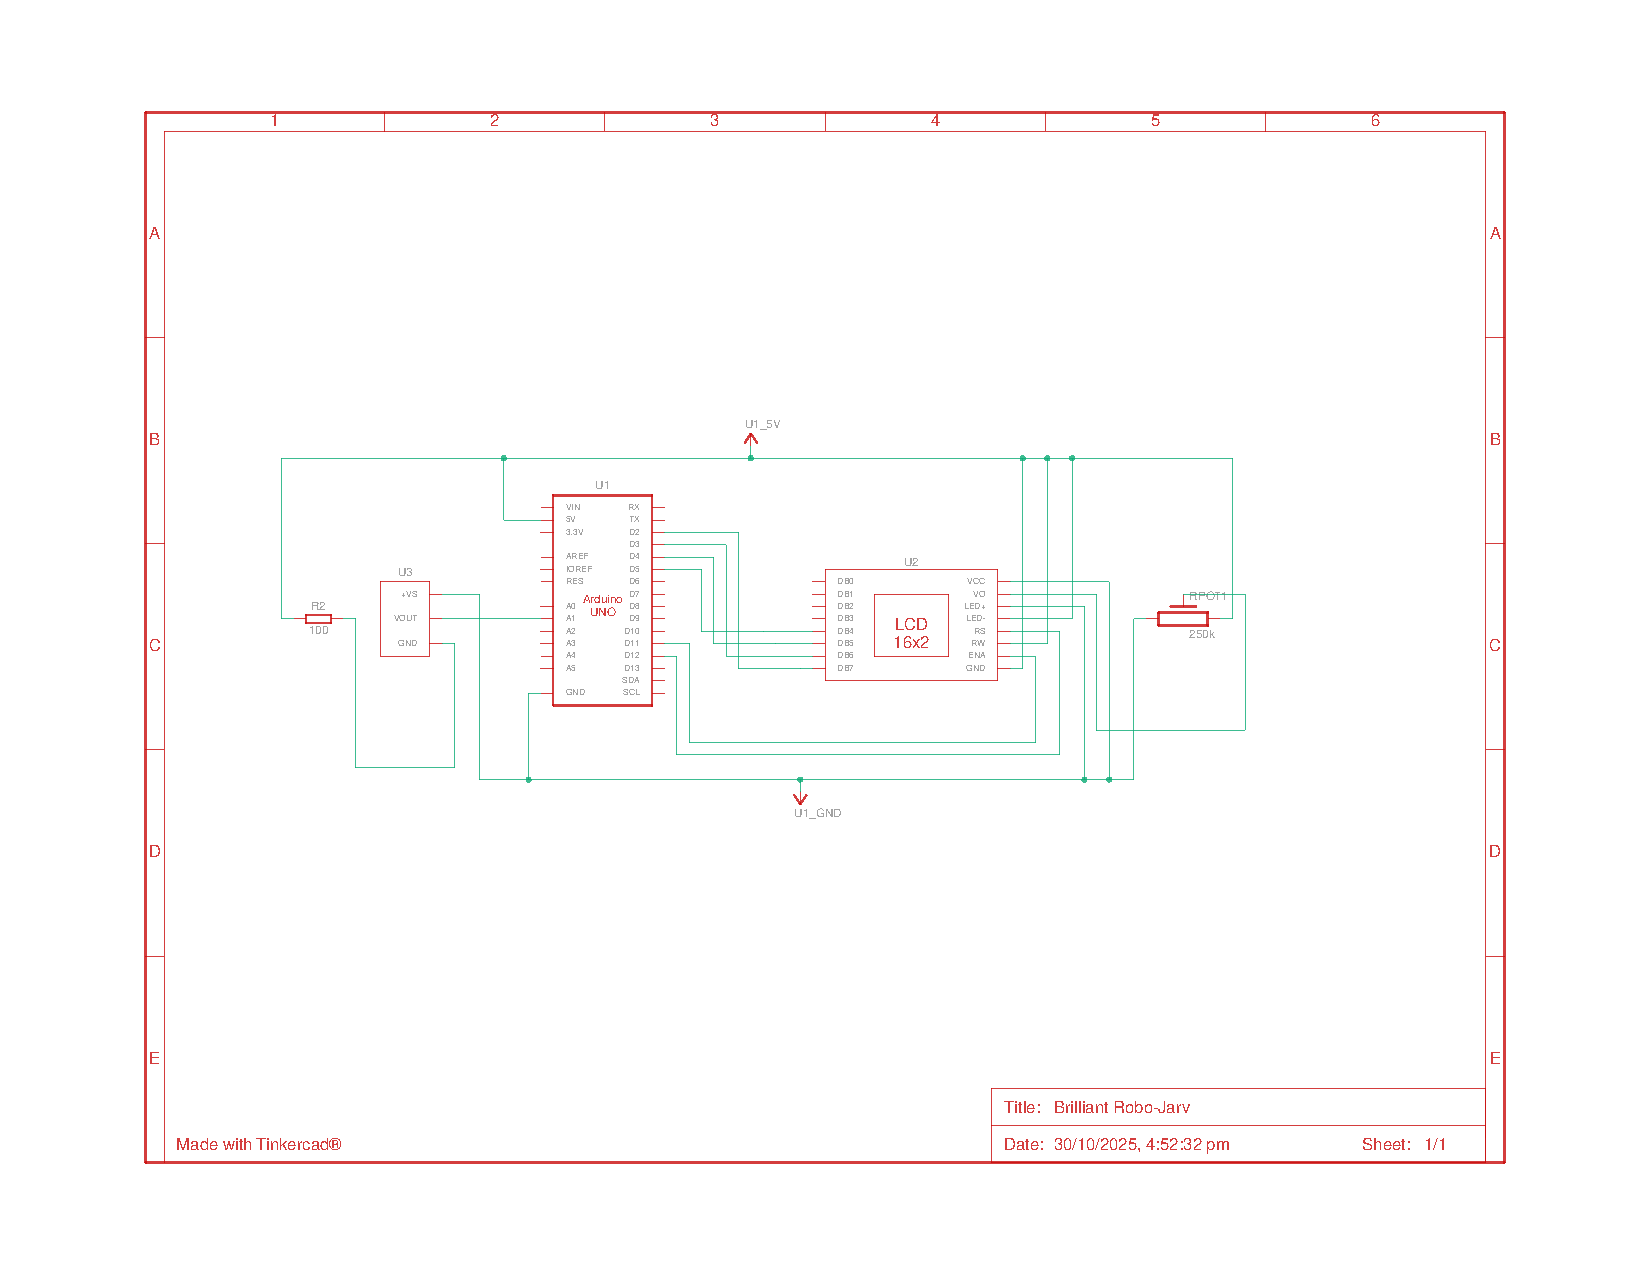
\includegraphics[width=0.9\linewidth]{figs/circuit.pdf}
    \caption{Circuit}
    \label{fig:placeholder}
\end{figure}
\newpage
\begin{figure}[h]
    \centering
    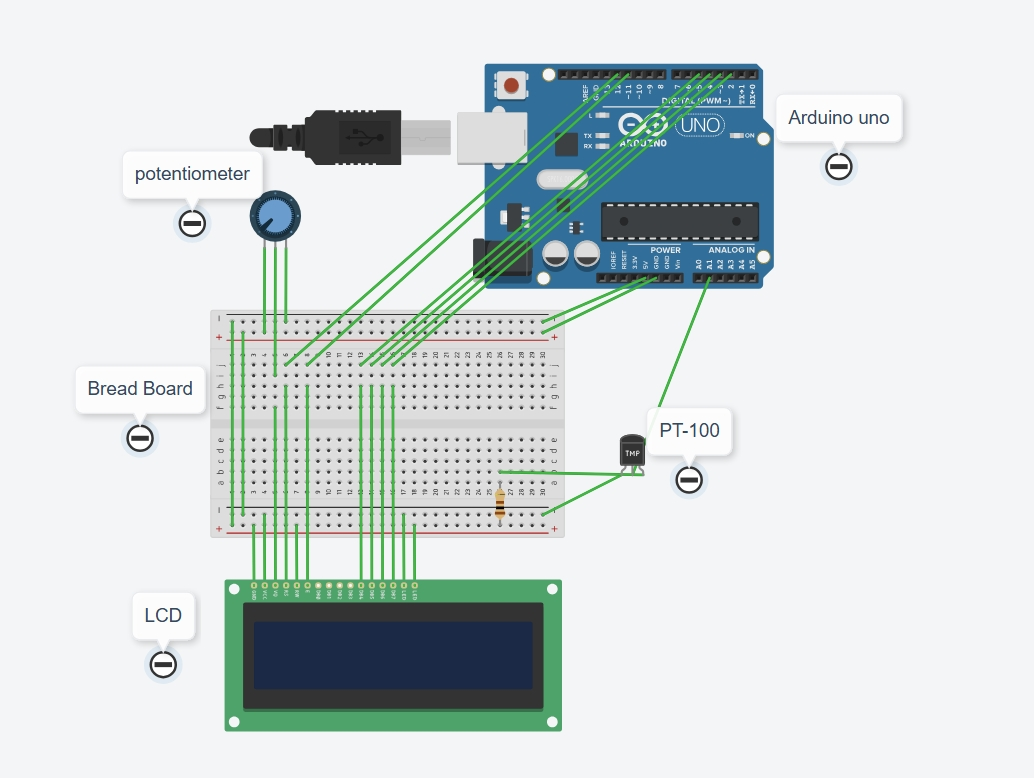
\includegraphics[width=0.5\linewidth]{figs/WhatsApp Image 2025-10-31 at 2.06.29 PM.jpeg}
    \caption{Circuit}
    \label{fig:placeholder}
\end{figure}
\newpage
\begin{figure}[h]
    \centering
    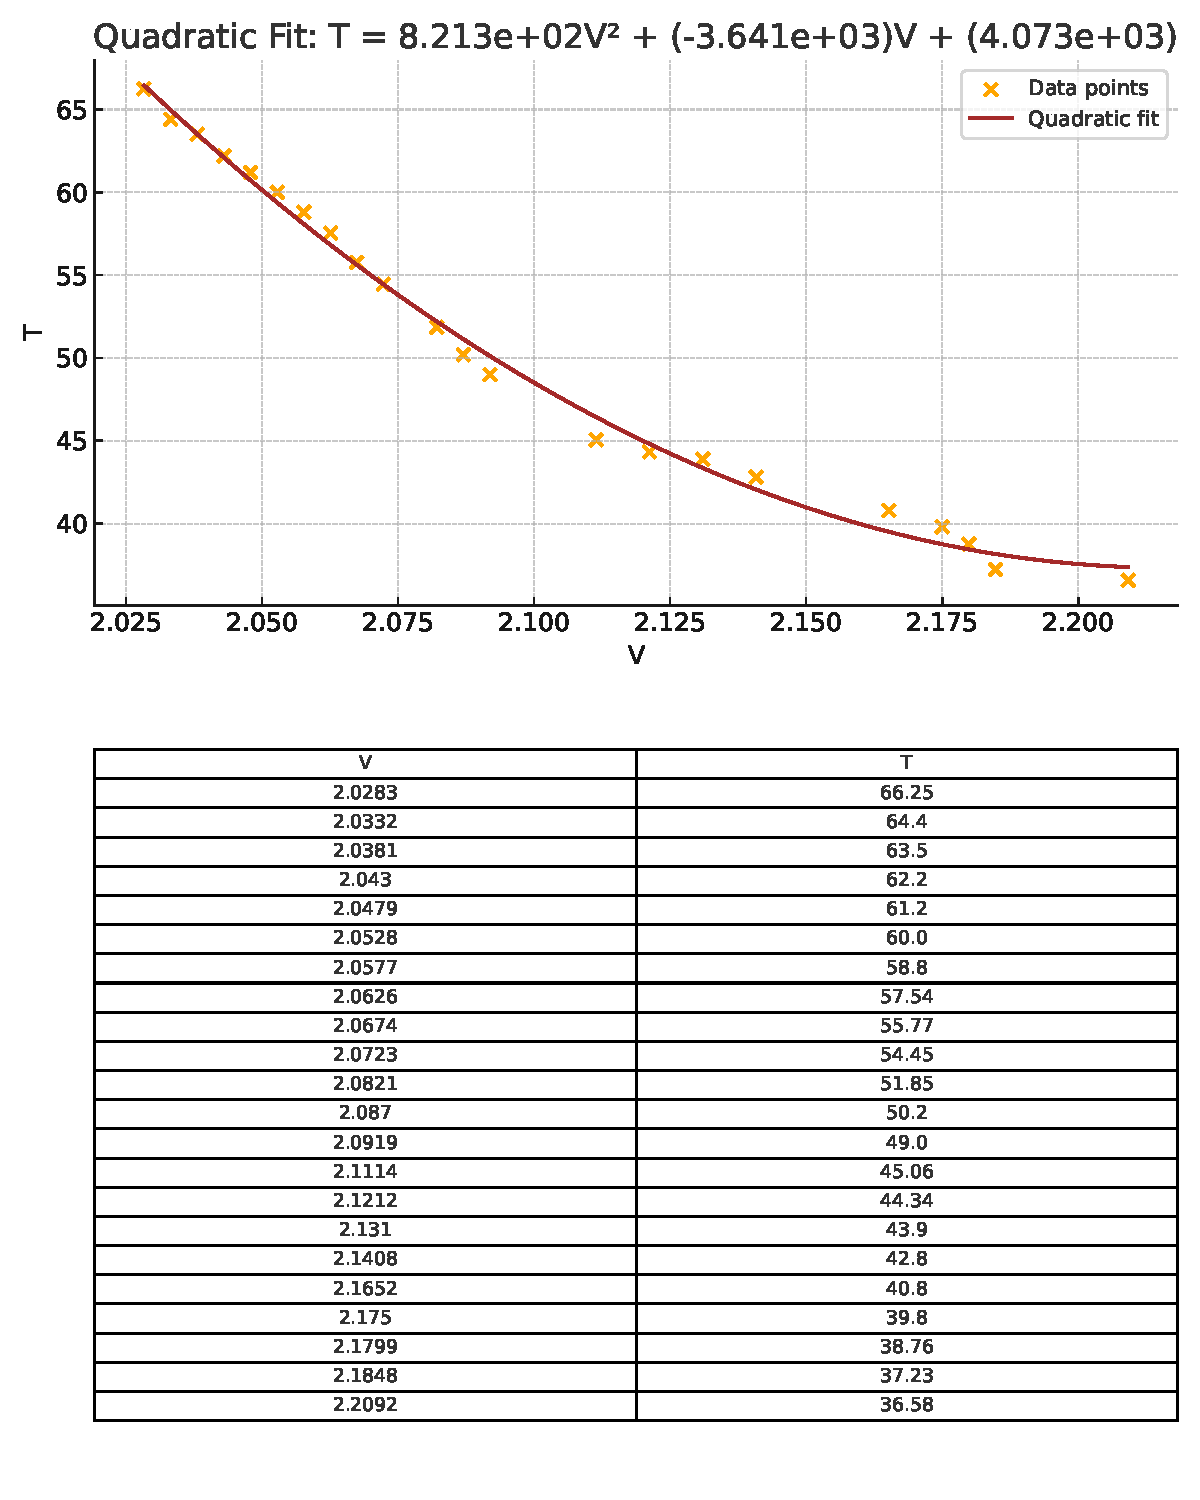
\includegraphics[width=0.9\linewidth]{figs/training data.pdf}
    \caption{training data}
    \label{fig:placeholder}
\end{figure}
\newpage
\section*{Method of Solving to find coefficients:}

Let the measured data points be $(T_i, V_i) ; i = 1,2, \ldots , n$

Callendos van dusen equation
\[
V = n_0 + n_1T + n_2T^2
\]

In matrix form
\[
C = Xn
\]
where
\[
C = \begin{pmatrix}
V_1 \\
V_2 \\
\vdots \\
V_n
\end{pmatrix}, \quad
X = \begin{pmatrix}
1 & T_1 & T_1^2 \\
1 & T_2 & T_2^2 \\
\vdots & \vdots & \vdots \\
1 & T_n & T_n^2
\end{pmatrix}, \quad
n = \begin{pmatrix}
n_0 \\
n_1 \\
n_2
\end{pmatrix}
\]

In linear regression we tend to minimize the sum of squared residuals
\[
E(n) = \|C - Xn\|^2 = (C - Xn)^T (C - Xn)
\]

\[
= (C^T - n^T X^T)(C - Xn)
\]

\[
= C^T C - C^T Xn - n^T X^T C + n^T X^T Xn
\]

We want
\[
\frac{d(E(n))}{dn} = 0
\]

\[
n = (X^T X)^{-1} X^T V
\]

we got
\[
\begin{pmatrix}
n_0 \\
n_1 \\
n_2
\end{pmatrix}
=
\begin{pmatrix}
2.773782 \\
-2.5304082 \times 10^{-2} \\
1.5400372 \times 10^{-4}
\end{pmatrix}
\]

For \[
T = a_0 + a_1 V + a_2 V^2
\]

we got
\[
\begin{pmatrix}
a_0 \\
a_1 \\
a_2
\end{pmatrix}
=
\begin{pmatrix}
4026.380134 \\
-3597.164799 \\
810.934776
\end{pmatrix}
\]
\begin{figure}[h]
    \centering
    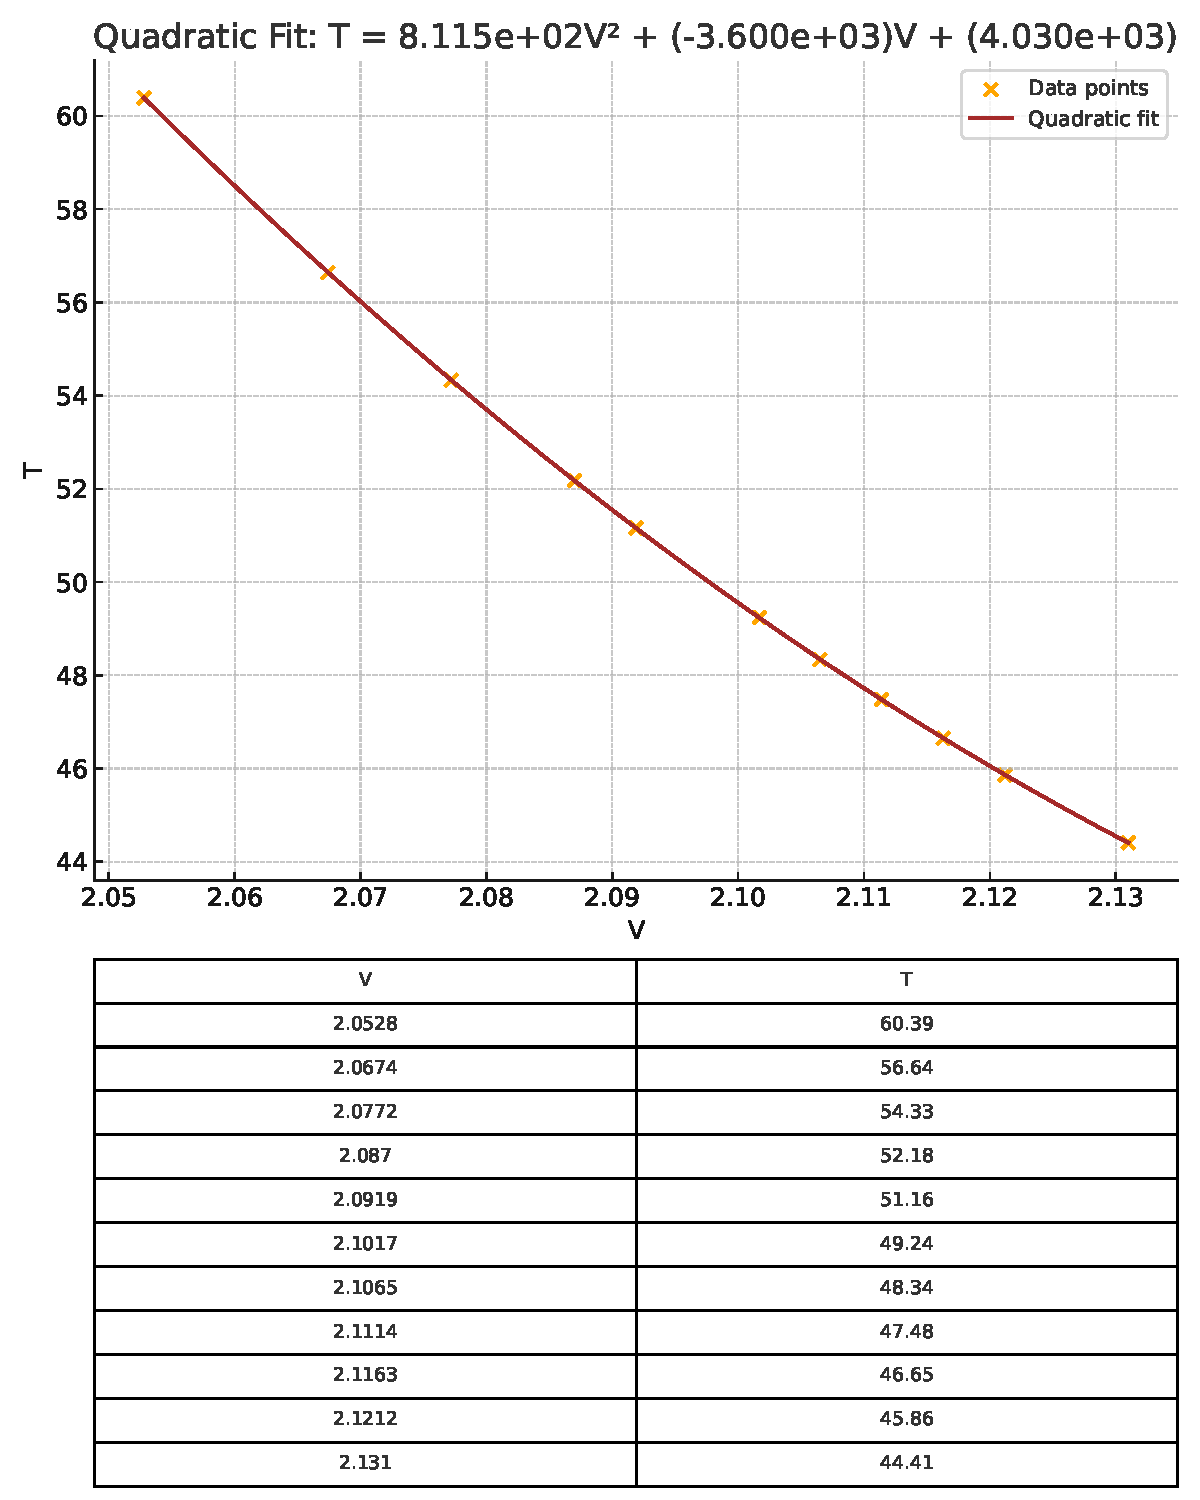
\includegraphics[width=0.9\linewidth]{figs/testing data.pdf}
    \caption{testing data}
    \label{fig:placeholder}
\end{figure}
\newpage
\section*{Calculating error:}

By Mean Absolute essor (M.A.E) for 10 data points
\[
MAE = \frac{\sum_{i=1}^{10} |T_i - T_i'|}{10}=2.511
\]

where

$T_i$ = Temperature by model \\
$T_i'$ = Temperature by thermometer


\section*{Performance of model:}

The model is moderate - good with deviation of $2.5^\circ C$.

\section*{Source of essors:}

\begin{enumerate}
    \item availability of poor quality and defect materials.
    \item providing small data set to model.
    \item Human essors while measuring.
    \item Approximation essors in the least squaees method.
    \item Sensor material uncertainties.
\end{enumerate}
\section*{\large{Arduino Code}}

\begin{verbatim}
#include <LiquidCrystal.h>

// Initialize LCD with pin numbers: RS, E, D4, D5, D6, D7
LiquidCrystal lcd(12,11,5,4,3,2);

float a0 = 4026.380134;
float a1 = -3597.164799;
float a2 = 810.934776;

// Pin definitions
const int PT100_PIN = A0;

// Constants for PT100 and voltage divider
const float VCC = 5.0;

//Calibration Parameters (Adjust after Calibration)
float offset = 0.0;
float sensitivity = 10.0;

void setup() {
  Serial.begin(9600);

  // Initialize LCD, 16 columns and 2 rows
  lcd.begin(16,2);

  // Display startup message
  lcd.print("PT100 Temp");
  lcd.clear();
}

analogReference(DEFAULT);

void loop() {

  // Read analog value from voltage divider
  int adcValue = analogRead(PT100_PIN);

  // Convert ADC value to voltage
  float voltage = (adcValue*VCC)/1023.0;

  // float temperature = a0 + a1*voltage + a2*voltage*voltage;
  //Calibrating the temperature by lcd
  float temperature = (temperature*sensitivity) + offset;

  // Show temperature on LCD
  lcd.clear();
  lcd.setCursor(0,0);
  lcd.print("Temp: ");
  lcd.print(temperature,2);

  lcd.setCursor(0,1);
  lcd.print("V: ");
  lcd.print(voltage,4);

  delay(1000);

}
\end{verbatim}
\section*{\large{linear regession code}}

\begin{verbatim}
import numpy as np

T = np.array([66.25, 64.40, 63.50, 62.20, 61.20, 60.00, 58.80,
57.54, 55.77, 54.45, 51.85, 50.20, 49.00, 45.06, 44.34,
43.90, 42.80, 40.8, 39.80, 38.76, 37.23, 36.58])

V = np.array([2.0283, 2.0332, 2.0381, 2.0430, 2.0479,
2.0528, 2.0577, 2.0626, 2.0674, 2.0723, 2.0821, 2.0870,
2.0919, 2.1114, 2.1212, 2.1310, 2.1408, 2.1652, 2.1750,
2.1799, 2.1848, 2.2092])

# V = n0 + n1 T + n2 T^2
X = np.vstack([np.ones_like(T), T, T**2]).T
n = np.linalg.lstsq(X, V, rcond = None)[0]
n0, n1, n2 = n
print("voltage model: V(T) = {:.6f} + {:.6f}T + {:.6f}T^2".
format(n0, n1, n2))

# T = a0 + a1 V + a2 V^2
X_inv = np.vstack([np.ones_like(V), V, V**2]).T
coeffs_inv = np.linalg.lstsq(X_inv, T, rcond = None)[0]
a0, a1, a2 = coeffs_inv
print("temperature model: T(V) = {:.6f} + {:.6f}V + {:.6f}V^2"
.format(a0, a1, a2))
\end{verbatim}
\centering{\textbf{THE END}}
\end{document}
